\section{医学视频数据预处理与优化}\label{sec:2}

对X线检查得到的DR图像进行预处理是计算机辅助诊断中的重要课题。为衡量生物器官对X射线的吸收率,Hounsfield\cite{peeters1979nobel}定义了描述辐射密度的标准量化单位。CT值的单位被命名为亨氏单位(Hounsfield Unit,简称Hu),以纪念Hounsfield为CT成像所作出的卓越贡献。CT值的计算公式如下:
\begin{equation}
    CT值 = \frac{\mu_m - \mu_w}{\mu_w} \times \alpha
\end{equation}
其中 $\alpha$ 为分度因子。当值取1000时,CT值的单位即为亨氏单位。$\mu_m$ 表示X射线穿透生物组织的衰减系数,而 $\mu_w$ 则代表标准水的衰减系数。亨氏单位将水的衰减系数作为标准,人体各种组织具备不同的衰减系数。在医学图像上,人体组织的 CT值范围一共有2000个单位。在这一数值之中,水的CT值位列中心点,数值为 \SI{0}{\Hu};空气的CT值最低,为 \SI{-1000}{\Hu};骨骼组织的CT值则最高,可达 \SI{1000}{\Hu}。CT值所涵盖的2000个单位远超过了灰度图像所能展现的范围,人眼无法直观分析原始的DR图像。针对某一特定组织,调窗技术可以提供更佳的可视效果,有助于更准确地观察病变区域与标志物范围。人们一般通过调整窗口中心和窗口宽度来完成从 CT 值到显示值的线性转换。窗口宽度指定组织的 CT 值范围,窗口中心指定组织 CT 值范围的中心。调窗技术只是令显示效果让人眼接受,并未对图像的原始信息进行更改。调窗技术对于计算机辅助诊断系统非常重要,为每类图像校准生成一致的对比度和特定的CT中心值。

\subsection{自动窗宽窗位算法}\label{sec:2_1}

本课题所分析的医学视频为受试者的侧位头部及颈部的DR图像。鉴于数据获取过程中,受试者未紧贴采集设备,且在吞咽钡餐时头部运动幅度显著,导致各组数据的累计灰度分布差异较大。因此,有必要对每组数据进行单独的窗宽窗位校正。
\begin{figure}[!htp]
    \centering
    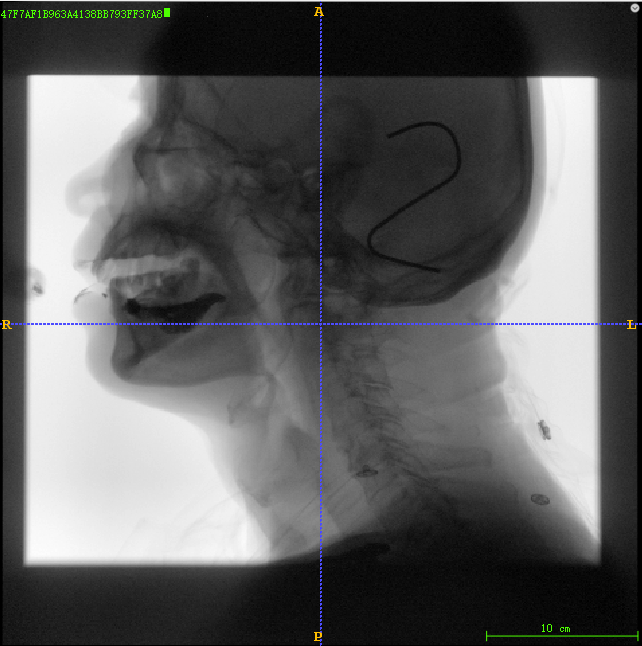
\includegraphics[width=0.4\textwidth]{figures/2_1_1.png}
    %\hspace{1cm}
    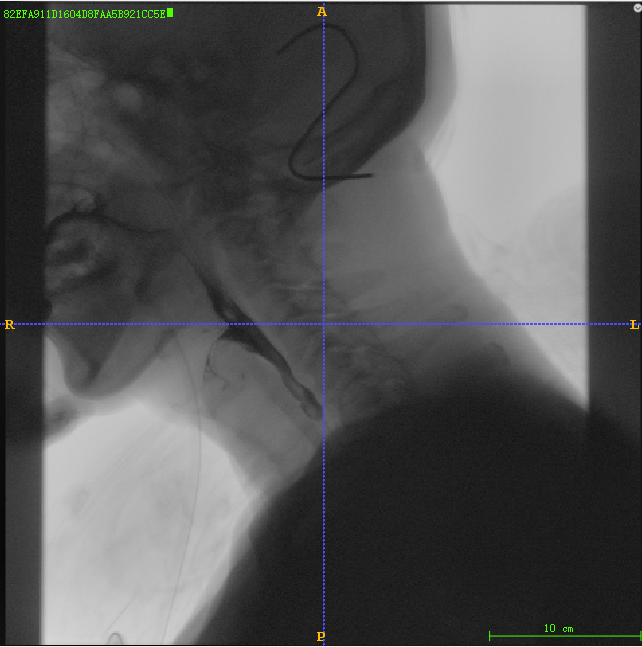
\includegraphics[width=0.4\textwidth]{figures/2_1_2.png}
    \caption{灰度分布差异较大的两组数据的帧截图}
    \label{fig:2_1_原始图像}
\end{figure}

\subsubsection{算法流程}

由于本实验所关注的对象(造影剂)并非人体器官或已被研究的细胞,且在时域中变化较为剧烈,没有已知公认推荐的窗位和窗宽。而人工对每组数据进行矫正耗时较大,且缺乏客观统一的评判标准。因此,本研究采用了基于累积分布函数的自动窗宽窗位算法。基于累积分布图,我们有以下两个普遍假设:
\begin{itemize}
    \item 分布函数的斜率变化反映了整幅图灰度值变化的快慢情况。
    \item 分布函数的斜率越大说明整幅图像的灰度分布越压缩,反之,说明灰度分布宽度越大。
\end{itemize}

最终,本研究采用以下步骤获取窗宽和窗位:
\begin{itemize}
    \item 从视频中划分出我们感兴趣的区域(喉口和咽部)。在本研究中,该步骤被简化为将视频按固定坐标的矩形裁剪。
    \item 从帧序列中等间隔地提取K张的帧图像。在本研究中,K固定为10。
    \item 对提取出的每张帧图像以 $\frac{1}{K}$ 的权重叠加,得到平均图像。
    \item 对平均图像求取累计分布序列 $S(x)$。即:图像中像素值小于等于 $x$ 的像素总数占图像总像素数的占比为 $S(x)$。
    \item 设定一组阈值区间 $[t_{min}, t_{max}]$。对于所有使得 $S(x)$ 落入阈值区间的 $x$,记录其坐标 $(x, S(x))$ 所形成的集合。在本研究中,$t_{min}$ 固定为0.05,$t_{max}$ 固定为0.95。
    \item 对于上述坐标集合,使用最小二乘法求得拟合直线 $y=kx+b$。
    \item 求得窗位为 $\frac{1-2b}{k}$,窗宽为 $\frac{1}{k}$。
\end{itemize}

\subsubsection{结果}

\cref{fig:2_1_对比} 展示了两组基于上述自动窗宽窗位算法处理前后的对照数据。这两组数据源自不同的受试者,且钡餐位于受试者体内不同位置。可以看出,本研究所使用的算法具有良好的适应性和稳定性。

\begin{figure}[!htp]
    \centering
    \begin{subfigure}{\textwidth}
        \centering
        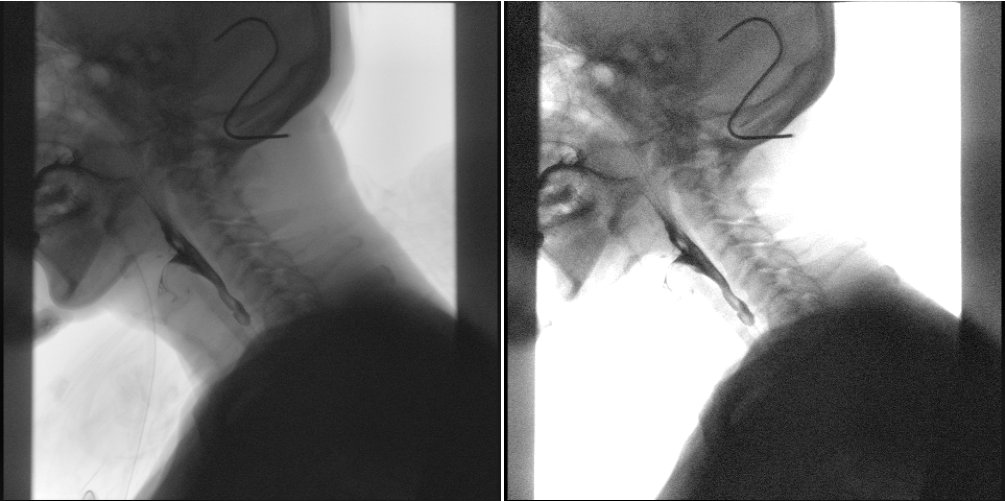
\includegraphics[width=\textwidth]{figures/2_2_1.png}
        \caption{受试者A}
    \end{subfigure}
    
    \begin{subfigure}{\textwidth}
        \centering
        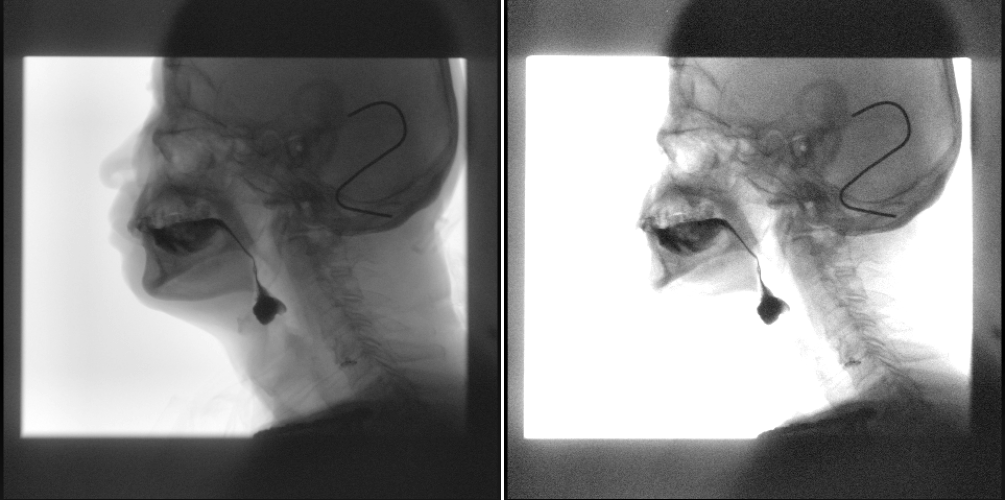
\includegraphics[width=\textwidth]{figures/2_2_2.png}
        \caption{受试者B}
    \end{subfigure}
    \caption{自动窗口算法应用前后对比}
    \label{fig:2_1_对比}
\end{figure}

\subsection{使用光流法配准}\label{sec:2_2}

在本研究的后续章节中,相邻帧图像的差值被用作求钡餐轮廓区域的重要基准。因此,我们需要先对每一帧图像进行配准。

医学图像配准旨在为一幅医学图像寻找一种或多种空间变换,以使其与另一幅医学图像的对应点在空间位置和解剖结构上达到完全吻合\cite{shi2017}。医学图像配准一直以来都是医学图像分析领域的研究热门话题。在众多方法中,基于光流的配准技术成为一种重要的形变配准方式\cite{ji2017based}。

光流概念最早源于计算机视觉领域,其模型可用于表现物体在观测成像平面上像素运动的瞬时速度。图像中每个像素点的运动速度与运动方向所构成的速度场,便被称为光流场。对图像应用光流法,需保证亮同一目标在不同帧间运动时,其亮度不会发生改变。在本课题中,我们主要使用了 Bouguet 和 Jean-Yves 提出的基于金字塔分层的LK光流法\cite{bouguet2001pyramidal}。传统的LK光流法应用在运动速度较快(即相邻帧之间对象的位移较大)的物体上时误差较大。而金字塔LK光流算法利用图像金字塔的多尺度特性,对不同尺度下的图像进行光流估计,从而提高光流估计的准确性和稳定性。

\subsubsection{算法流程}

假设 $u$ 是图像 $I$ 中的一个点,我们要在图像 $J$ 中找到它对应的点 $v$,及对应的变换矩阵 $A$。算法简要流程如下:
\begin{itemize}
    \item 建立 $I$ 和 $J$ 的图像金字塔 \; $\{I^L\}_{L=0,\cdots,L_m} \text{ and } \{J^L\}_{L=0,\cdots,L_m}$
    \item 初始化金字塔上的位移估计为0 \; $\textbf{g}^{L_m}=[g_{x}^{L_m} \; g_{x}^{L_m}]^T=[0 \; 0]^T$
    \item 对 $L_m$ 到 $L_0$ 中的每一个 $L$:
    \subitem 找到 $u$ 在图像 $I^L$ 中的位置 \; $\textbf{u}^L=[p_x \; p_y]^T=\frac{\textbf{u}}{2^L}$
    \subitem 计算 $I^L$ 对 $x$ 的导数 \; $I_x(x,y)=\frac{I^L(x+1,y)-I^L(x-1,y)}{2}$
    \subitem 计算 $I^L$ 对 $y$ 的导数 \; $I_y(x,y)=\frac{I^L(x,y+1)-I^L(x,y-1)}{2}$
    \subitem 计算空间导数矩阵 \; $G=\sum_{x=p_x-\omega_x}^{p_x+\omega_x} \sum_{y=p_y-\omega_y}^{p_y+\omega_y} \begin{bmatrix} I_x^2(x,y) & I_x(x,y)I_y(x,y) \\ I_x(x,y)I_y(x,y) & I_y^2(x,y) \end{bmatrix} $
    \subitem 初始化L-K迭代。对 1 到 $K$ 中的每一个 $k$:
    \subsubitem 图像相减 \; $\delta I_k(x,y)=I^L(x,y)-J^L(x+g_x^L+\nu_x^{k-1},y+g_y^L+\nu_y^{k-1})$
    \subsubitem 计算图像误匹配向量 \; $\overline{b}_k=\sum_{x=p_x-\omega_x}^{p_x+\omega_x} \sum_{y=p_y-\omega_y}^{p_y+\omega_y} \begin{bmatrix} \delta I_k(x,y)I_x(x,y) \\ \delta I_k(x,y)I_y(x,y) \end{bmatrix} $
    \subsubitem 计算光流 \; $\overline{\eta}^k=G^{-1}\overline{b}_k$
    \subsubitem 累加迭代量 \; $\overline{\nu}^k = \overline{\nu}^{k-1} + \overline{\eta}^k$
    \subsubitem 若 $||\overline{\eta}^k||$ 小于设定阈值,打断迭代
    
    \subitem 得到第 $L$ 层的光流估计 \; $\textbf{d}^L = \overline{\nu}^K$
    \subitem 计算出 $L-1$ 层的初步估计 \; $\textbf{g}^{L-1}=[g_x^{L-1} \; g_y^{L-1}]^T=2(\textbf{g}^L+\textbf{d}^L)$
    \item 得到最终的光流估计 \; $\textbf{d}=\textbf{g}^0+\textbf{d}^0$
    \item 定位图像J中的位置 \; $\textbf{v}=\textbf{u}+\textbf{d}$
\end{itemize}

\subsubsection{结果}

\cref{fig:2_2_对比} 展示了一组基于上述光流法处理前后的对照数据。
\clearpage
\begin{figure}[!htp]
    \centering
    \begin{subfigure}{\textwidth}
        \centering
        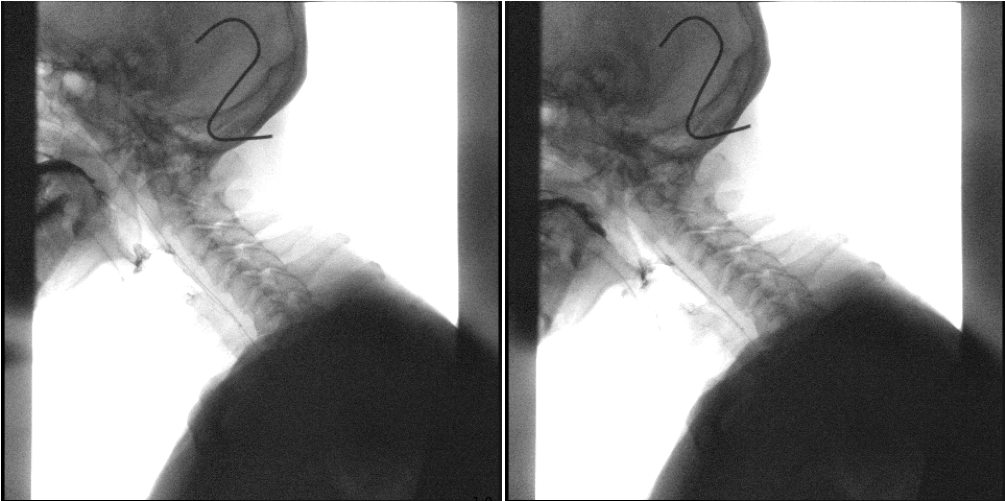
\includegraphics[width=\textwidth]{figures/2_3_1.png}
        \caption{一组数据中的两帧原始图像}
    \end{subfigure}
    
    \begin{subfigure}{\textwidth}
        \centering
        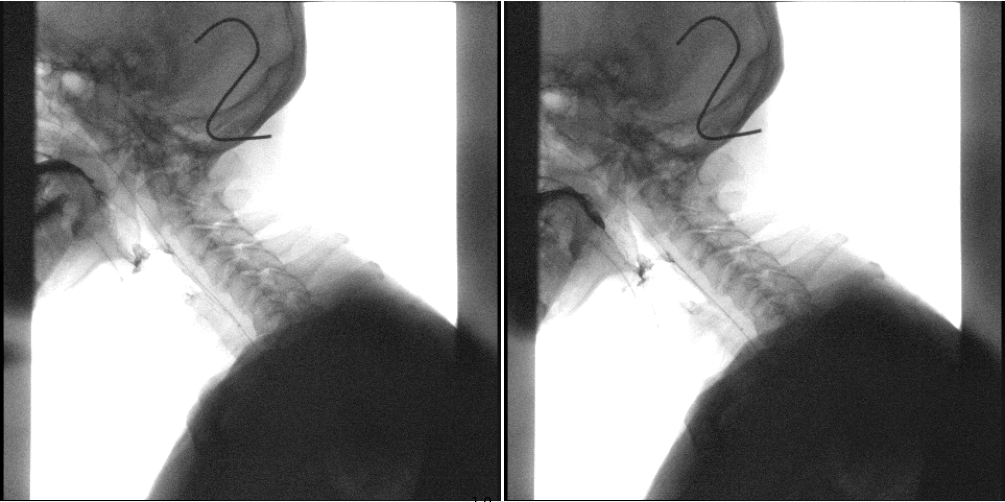
\includegraphics[width=\textwidth]{figures/2_3_2.png}
        \caption{经光流法配准后的两帧图像}
    \end{subfigure}
    \caption{光流法应用前后对比}
    \label{fig:2_2_对比}
\end{figure}

可以看出,该算法抵消了部分受试者的头部运动,为后续逐帧图像分析处理提供正向作用。

\subsection{本章小结}

本章将对待处理的视频数据进行预处理。首先运用自动窗宽窗位算法,凸显出我们所关注的感兴趣区域;接着从数据中提取运动形态变化信息,并采用光流法对图像进行配准,为后续逐帧图像分析处理奠定基础。